\documentclass[symmetric, a4paper, 11pt]{article}
\title{Migovec Science Project}

\author{Tanguy Racine Imperial College Caving Club}
\usepackage{grffile}
\usepackage{caption}
\usepackage
{ccaption}
\usepackage{subcaption}
\captionsetup{compatibility=false}
\usepackage{graphicx}
\usepackage[utf8]{inputenc}
\usepackage{helvet}
\usepackage{multicol}
\usepackage{ragged2e}
\usepackage{cite}
\usepackage{xcolor}
\usepackage{pagecolor}
\usepackage[pages=some,placement=center]{background}
\usepackage{afterpage}
\usepackage{booktabs}
\usepackage{colortbl}
\usepackage{tabularx}
\usepackage{multirow}
\usepackage[strict]{changepage}



\begin{document}
\maketitle

\section{Introduction}
Caves are important markers of surface morphological evolution: the presence of  horizontal levels are generally thought as markers of ancient base levels. By means of indirect dating of the cave sediments and speleothems, the age of those systems can be determined. Methods include U/Th dating of speleothems, palaeontology, palynology,  cosmogenic dating of sediment and palaeomagnetic studies. To be useful, such mehtodologies must be incorporated within a speleogenetic framework.  Sistem Migovec  in the Julian Alps (explored 1976 to present) is an unusually complex and long alpine system belonging to the 3D network of vadose shaft and phreatic galleries.  Since sub-horizontal to horizontal levels  are generally tied to the valley bottoms, they represent periods of erosional still stand or  erosional events. The deliverables of a comprehensive speleogenetic and dating study are a constrained history of climate change and uplift south of the Peri-Adriatic line, in the Julian Alps. 

\section{Motivation}
Sistem Migovec is a 39.3km long cave system, lying in the Triglav National Park, NW Slovenia. It comprises 8 entrances, contains 5 horizontal levels,  and >10 distinct shaft series, not all connected, which take the diffuse recharge on a morphologically complex plateau. The cave is formed in the upper Triassic limestone of the Dachstein formation, which now comprise part of the Slatna overthrust, a SW verging, mostly carbonate thrust sheet mobilised during the Alpine and later Dinaride orogenies. Tectonic activity in the region is ongoing, as evidenced by the 1998 Ravne earthquake. Horizontal levels show most of the signs of being relict phreatic trunk passages, reaching between 5-15m in width, and later infill by sediment. Other sedimentary deposits along the cave walls, solution pockets and smaller inlet phreatic tubes  suggest at least one stage of rejuvenation, and vadose undercutting of the sediment pile and wall rock underneath. With the highest horizontal levels at 1600m asl, about 1100m above present day base level in the Tolminka valley, and lower levels evenly distributed in depth, there is  unique potential for a detailed and insightful landscape evolution dynamics study in this area of the southern Julian alps. Dye tracing experiments would likely help identify a resurgence: the deepest entered passages head towards the west side of mountain.

\begin{figure*}[t!]
\centering
\frame{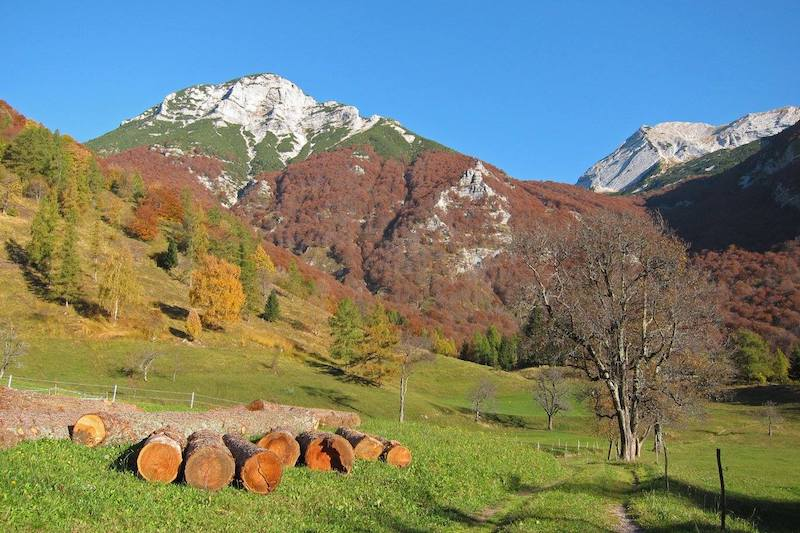
\includegraphics[width=\textwidth]{Migovec_in_Autumn.jpg}}
\caption{The southern face of Tolminksi Migovec, seen from the mountain village of Tolminkse Ravne (924m asl) --- Jana Čarga }
\label{water chamber below helm's deep}
\end{figure*}


    
\section{Potential methods of dating}
There is certainly some potential for palaeomagnetic work although a careful reconnaissance observation work would be needed to verify this, in particular I would need to identify a suitable sequence of magnetic observation sites over the 972m depth range of the cave so that it could be tied in to the magnetic reversal history. In the deep alpine system of Migovec, the depth range is sufficient to get a series of reversals but I would need first to ascertain the presence of Present Day sediments (those near sump level). This will  prove problematic given the conspicuous absence of horizontal levels in the epi-phreatic zone, and the absence of relict phreatic tubes infilled red clay (personal correspondence). In all probability, infill sediments are restricted to the upper 700m of the cave and without the present day sediments it is unlikely that a tied set of observations can be established. 

I think the use of of palynology would be a more direct and reliable method since it would require taking well located hand samples at a range of depths in the cave. Some locations could provide a >10m section into the sediment column.

In terms of dating speleothems, intial detailed observations at those regions of the cave that are more decorated will help identify some crucial deposits. 

\section{Maps and photographs}

 \begin{figure*}[h]
    \centering
    \includegraphics[width=\textwidth]{"MigKuk".jpg}
    \caption{The upper Triassic Dachstein limestones of Tolminksi Migovec (pink in geological map) have a gentle syncline geometry. On the left, a short glacial cirque leads to beheaded valley. Center, karstic processes dominate with long lines of dolines and collapse shakeholes}
    \end{figure*}
    
 \begin{figure*}[t!]
\centering
  \includegraphics[width=\textwidth]{"Geological map".png}
  \label{map m}
  \caption{A Slovenian government geological map of the area, Slovenian National Grid ESPG 3794}
 \end{figure*}
 
  \begin{figure*}[t!]
\centering
  \includegraphics[width=\textwidth]{"projections-mig".pdf}
  \label{map m}
  \caption{Projections of the main line surveys of the Migovec Cave System (2017)}
 \end{figure*}
    
 \begin{figure*}[t!]
\centering
  \includegraphics[width=\textwidth]{"elevation map".pdf}
  \label{map m}
  \contcaption{Cave passage and topography of Tolminski Migovec, Slovenian National Grid ESPG 3794}
 \end{figure*}
 

\begin{figure*}[t!]
\centering
  \includegraphics[width=\textwidth]{"Area M map".pdf}
  \label{map m}
  \caption{Topographic map of the Migovec Plateau with highlighted cave entrances. Slovenian National Grid ESPG 3794}
 \end{figure*}
 
\begin{figure*}[t]

    \centering
          
    \begin{subfigure}[t]{0.485\textwidth}
    \centering
        \frame{\includegraphics[width=\linewidth]{"Frost-crystals Leprechaun".jpg}} 
        \caption{} \label{Panorama}
    \end{subfigure}
        \hfill
        \begin{subfigure}[t]{0.485\textwidth}
        \centering
        \frame{\includegraphics[width=\linewidth]{"Frost-crystals-Leprechaun-2".jpg}} 
        \caption{} \label{Ice}
    \end{subfigure}
          \vspace{0cm}
          
    \begin{subfigure}[t]{0.355\textwidth}
        \centering
        \frame{\includegraphics[width=\linewidth]{"Frost-mud-formations".jpg}} 
        \caption{} \label{Will Scott bolting}
    \end{subfigure}
    \hfill
    \begin{subfigure}[t]{0.629\textwidth}
        \centering
        \frame{\includegraphics[width=\linewidth]{"Frost-mud-formations-2".jpg}} 
        \caption{} \label{Ice}
    \end{subfigure}

    \caption{
    \emph{a}   and  \emph{b} Calcite and aragonite needles in Leprechaun Passage
    \emph{c} Mud/clay formation in 'Potato Passage' 
    \emph{d} Calcified mud formations near 'Strap on the Nitro' Aven. --- Jarvist Frost}
\end{figure*}

\begin{figure*}[t!]
\centering
\includegraphics[width=\textwidth]{"Helm's deep".JPG}
\label{helm's deep}
\caption{A 15m high sediment pile infills one of the relict, trunk phreatic passages at depth of -750m --- Photo by Rhys Tyers}
\end{figure*}

\end{document}
